\section{Diseño}
A continuación se presentan y explican algunas de las decisiones de diseño elegidas durante el desarrollo del trabajo práctico.
Se decidió dividir la presentación en subsecciones para facilitar su comprensión, haciendo especial énfasis en aquellas que consideramos que son de mayor importancia.

%Vale mencionar que si bien es cierto que se genero una idea general en el grupo antes de comenzar a reflejar las decisiones tomadas en codigo, el diseño en profundidad se termino de desarrollar y afinar en paralelo, mientras surgian cuestiones mismas relacionadas al propio desarrollo que no habian sido tenidas en cuenta en papel. 


\subsection{Participantes, cap y fichas}
Decidimos que en un modelado correcto del participante, no se encontraba entre sus responsabilidades el conocer su cap (presupuesto para armar equipos) ni su cantidad de fichas disponibles, puesto que no son esenciales. Por lo tanto diseñamos dos clases, \textbf{GestorDeCap} y \textbf{GestorDeFichas}, cuyas instancias son objetos que conocen para un participante dado el cap y la cantidad de fichas disponibles, respectivamente, además de proveer un protocolo para la actualización de esos valores. De este modo, estas dos clases nos permiten desligar a las instancias de la clase Participante de dichas responsabilidades.\\
El nombre Gestor para ambas clases proviene del hecho de que sus instancias gestionan las fichas/caps de los participantes, no són solo objetos que proveen información, sino que la mantienen también.\\
Instancias de ambas clases se utilizan también en la gestión de desafíos: las apuestas afectan la cantidad de fichas disponibles de un participante para otros desafíos, al igual que el resultado de un desafío, y éste también afecta al cap del participante.\\
El GestorDeCap, entonces, utiliza también la clase Presupuesto, que representa en el contextor del Gestor al presupuesto máximo que un participante tiene como límite a la hora de conformar equipos.\\
Análogamente, el GestorDeFichas utiliza la clase Fichas, que representa una cantidad de fichas dada.\\
Si bien ambas clases parecen representar conceptos parecidos, preferimos organizar el conocimiento en dos clases distintas, para dejar en claro la diferencia existente entre ambas entidades en el dominio del problema.\\

\begin{center}
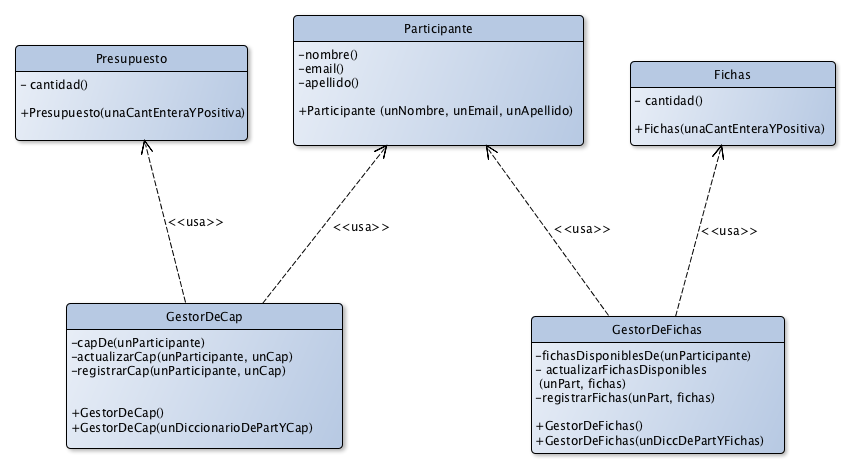
\includegraphics[scale=0.4]{diseno/gestorDeCapYFichas.png} 
\end{center}

Finalmente, con el mismo argumento esgrimido en párrafos anteriores, no es esencial al participante conocer directamente sus equipos. Resolvimos esto de una manera similar, como explicaremos en la siguiente subsección.\\


\subsection{Gestión de Equipos y Equipos}

\subsubsection{Gestor de Equipos}
Al no resultar esencial al participante conocer sus equipos, ni que el equipo conozca a su dueño/participante, resolvimos diseñar una clase cuyas instancias proveen un protocolo para obtener los equipos de un participante, al igual que crearlos, agregarlos y/o removerlos.\\
Este objeto, además, es el encargado de realizar las validaciones correspondientes a la hora de registrar un equipo para un participante. Es por esta razón que posee como colaboradores internos al GestorDeCap de la sección anterior (con el objetivo de no permitir la creación de equipos que superen el presupuesto de un participante), al igual que un objeto de la clase ListaPreciosJugador, encargado de conocer los precios de cada uno de los jugadores que viven en el modelo.\\
Esta última clase surgió también con un argumento similar a los expresados hasta ahora: no parecía ser ni esencial ni responsabilidad de un jugador conocer su precio, sino que era un dato que se podría consultar a otra entidad.\\

\begin{center}
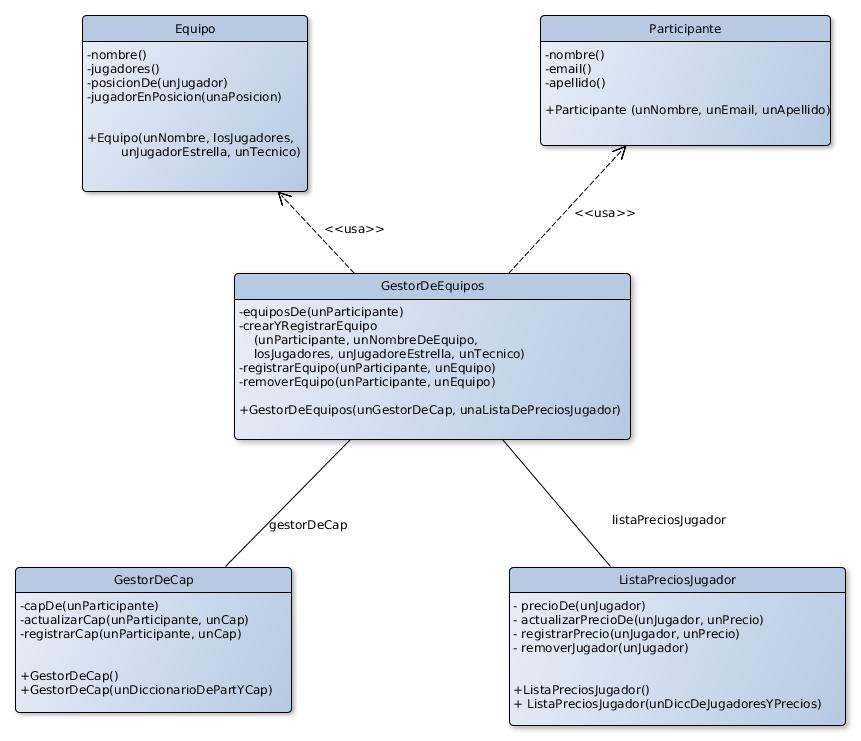
\includegraphics[scale=0.4]{diseno/gestorDeEquipos.jpg}
\end{center}

\subsubsection{Equipos}

Un equipo está conformado por sus cinco jugadores, uno de los cuales es un jugador estrella, y un técnico.
Lo primero a notar en nuestro modelado del equipo es que en realidad no debería ser esencial a un jugador conocer su posición. La razón es simple: la posición en la que un jugador juega en un equipo es un componente estratégico, que incluso podría tener efectos a la hora de simular un partido. Por esta razón, es el equipo quien conoce la posición de un jugador que forma parte del mismo. \\
Así, las instancias de la clases Equipo utilizarán las clases que subclasifican a la clase abstracta Posición. Modelar la posición con una jerarquía de clases cuyas instancias representarán los distintas posiciones, nos permitirá que un equipo pueda responder con facilidad mensajes que devuelvan en qué posición juega un jugador en el equipo o qué jugador juega en el equipo en una posición dada. \\
Esto resultó extremadamente útil a la hora de implementar la jugada defensiva Hombre a Hombre. Las posiciones y el equipo colaborarán en este caso en el contexto de una simulación haciendo uso del mecanismo de double dispatch, a fin de evitar la aparición de estructuras de control (como \textbf{if}) innecesariamente en el código fuente.\\
Además, de la misma manera en que no es responsabilidad de un jugador conocer su precio, tampoco lo es conocer sus estadísticas. Los objetos de la clase RegistroDeEstadisticas son quienes conocen las estadísticas de los jugadores, como veremos en secciones subsiguientes.\\
Finalmente, un técnico conoce su nombre, su apellido, su nombre completo y su libro de jugadas, representado con instancias de la clase LibroDeJugadas, que hará uso de las clases JugadasOfensivas y JugadasDefensivas, a la vez que mantiene la frecuencia con la que el técnico elige cada una de las jugadas. Estas clases se usarán a la hora de elegir jugadas defensivas u ofensivas para el equipo, según corresponda en el contexto de la simulación.\\

\begin{center}
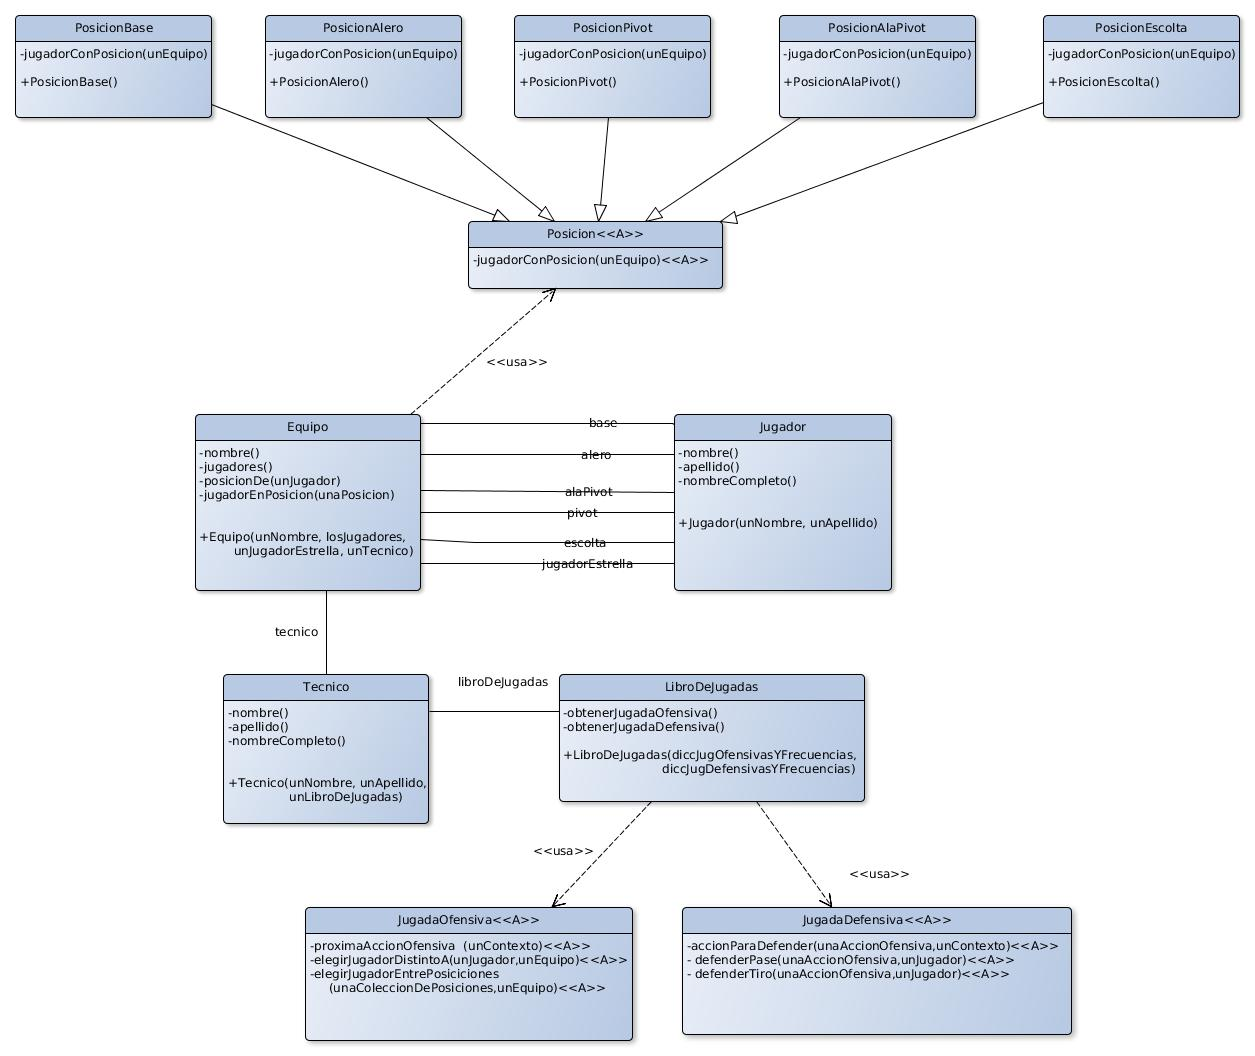
\includegraphics[scale=0.30]{diseno/equipo.jpg} 
\end{center}

\subsection{Registro de estadísticas}
Mencionamos en la sección anterior que no es responsabilidad de un jugador conocer sus estadísticas. Esta responsabilidad, entonces, recae en las instancias de la clase RegistroDeEstadísticas, que sabrán responder las estadísticas de un jugador dado, al igual que proveer un protocolo para actualizarlas.\\
El nombre de Registro tiene sentido si se lo piensa como una entidad donde se pueden consultar, registrar y mantener las estadísticas de un jugador.\\
Para ello, además, modelamos a las estadísticas como instancias de la clase Estadística, quien provee los mensajes necesarios para obtener los distintos valores necesarios del jugador. Lo interesante de modelarlo de este modo es que provee modificabilidad: en un futuro se podrán incorporar nuevos tipos de estadísticas para el jugador de básquet; bastará con subclasificar la clase existente y definir los métodos a agregar.\\

\begin{center}
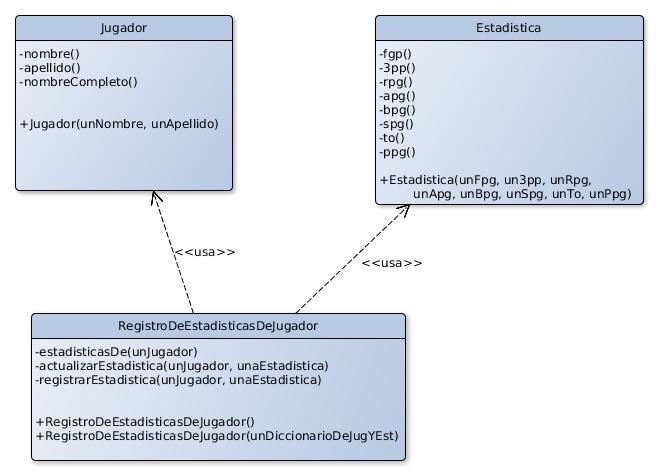
\includegraphics[scale=0.4]{diseno/registroDeEstadisticas.jpg}
\end{center}


\subsection{Acciones}

Diferenciamos principalmente dos tipos de acciones: las ofensivas, como lo son los pases y los tiros al aro, y las defensivas, como el bloqueo y la intercepción.
Hay además una acción especial, el rebote, que se utiliza cuando al simular el reboteo durante un turno y que no es ni ofensiva ni defensiva.\\
Modelamos esto mediante la jerarquía de clases de Acciones. La clase abstracta Acciones define un protocolo abstracto de mensajes: jugadorEjecutante() y resolvedorPara(self). El primero viene a cuento de que en nuestro modelado de acciones, una acción conoce quién la va a ejecutar. Una acción colaborará con un simulador, usando double dispatch, para definir el \textit{resolvedor} a usar para tal acción en el turno; el \textit{resolvedor} (mala traducción de \textit{solver}) es el objeto que conoce las ecuaciones de resolución de las acciones.\\
La clase abstracta Accion se subclasifica entonces en dos clases a su vez abstractas, AccionOfensiva y AccionDefensiva, y también en Rebote. Asimismo, la AccionOfensiva se subclasifica en Pase (que además del ejecutante de la acción sabe responder el receptor del pase), Tiro2Puntos y Tiro3Puntos; AccionDefensiva, en cambio, se subclasifica en Bloqueo e Intercepción.

\begin{center}
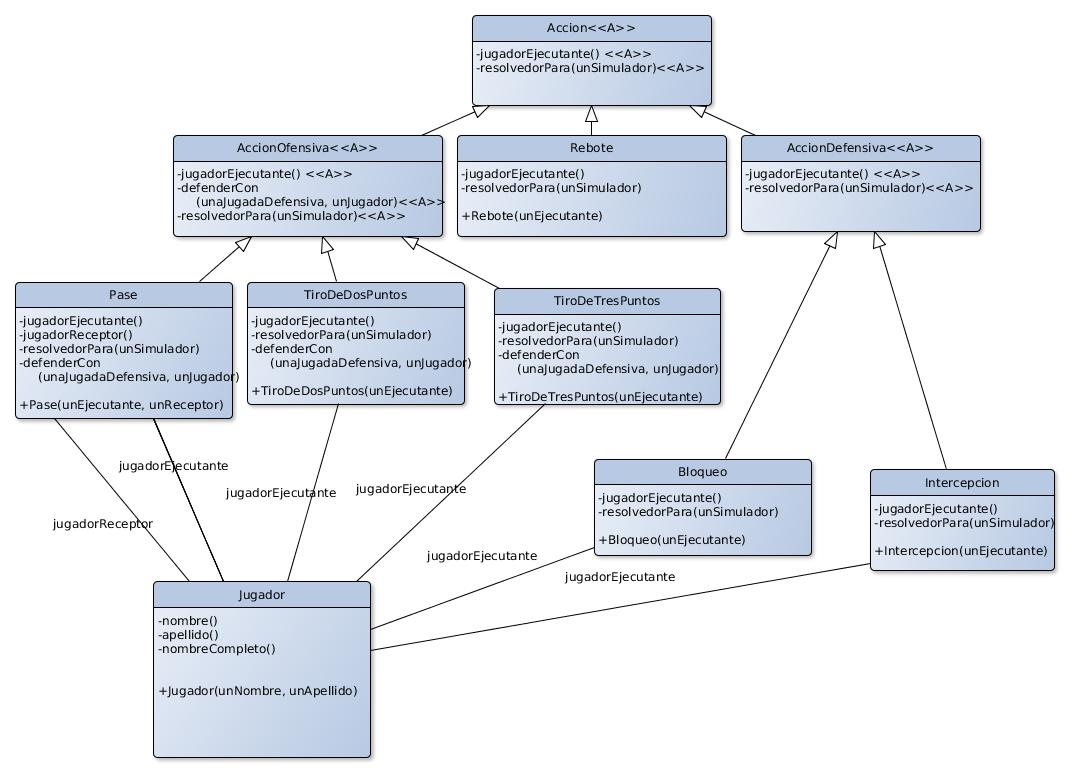
\includegraphics[scale=0.35]{diseno/acciones.jpg}
\end{center}

Mencionamos que un Simulador colabora con la acción para obtener su resolvedor correspondiente, que conoce las reglas de resolución de las acciones. El siguiente diagrama de clases muestra la relación entre el Simulador y los distintos Resolvedores.


\begin{center}
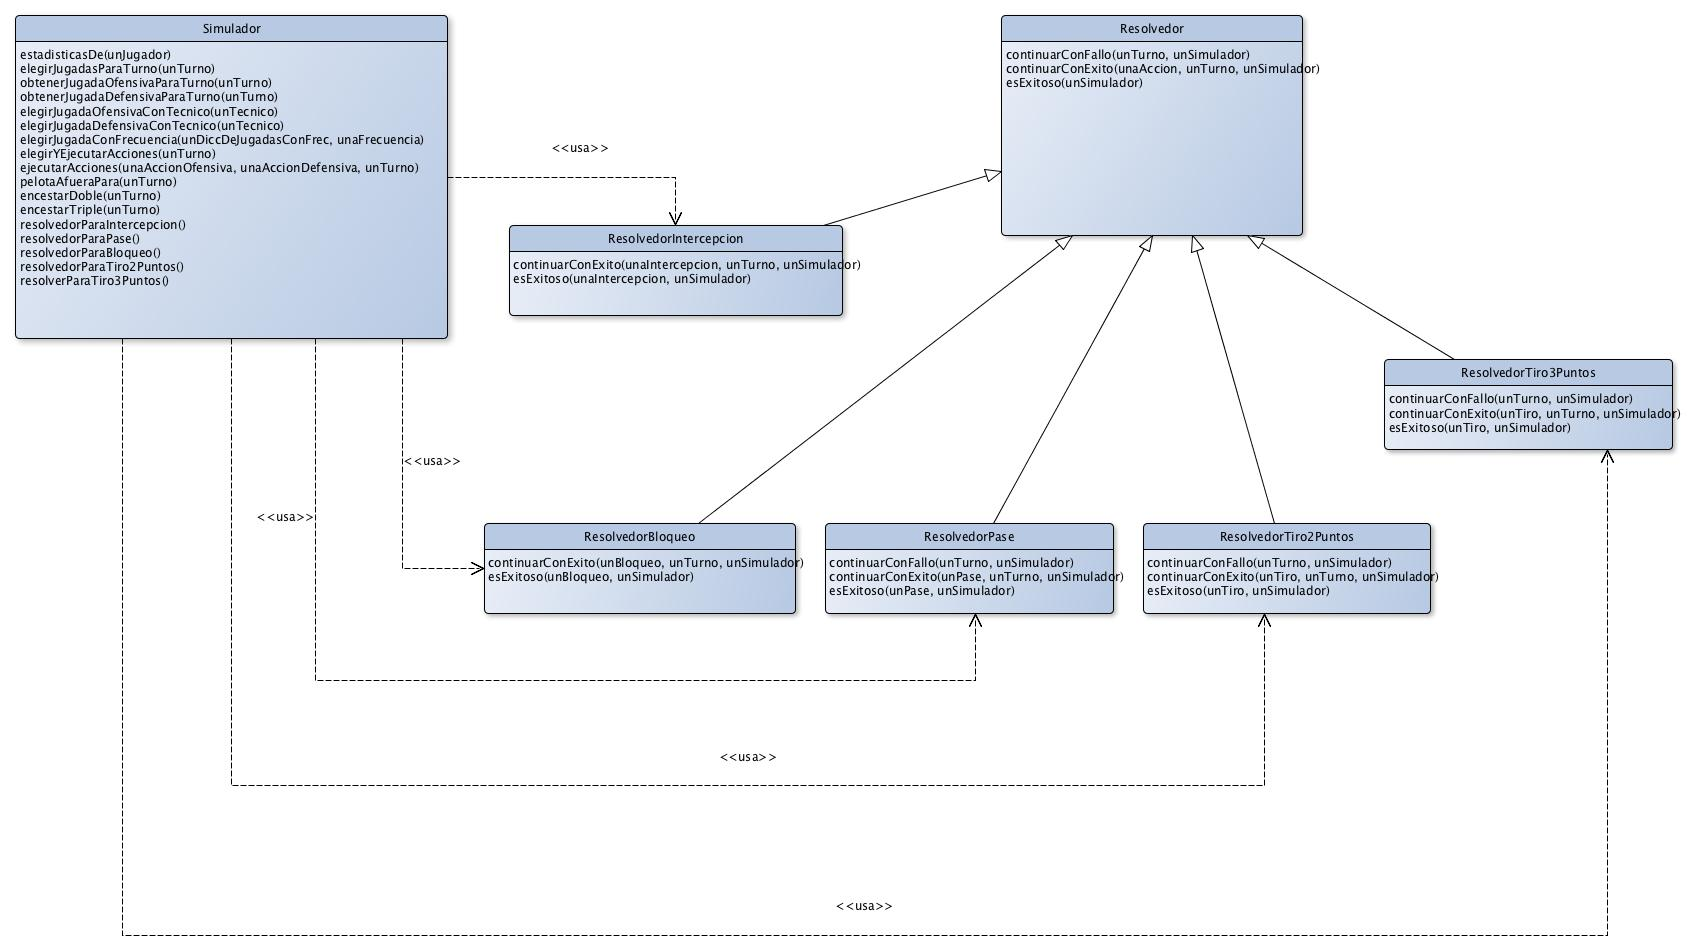
\includegraphics[scale=0.35, angle=90]{diseno/simuladorYResolvedor.jpg}
\end{center}

La clase abstracta Resolvedor representa a un resolvedor de acción, y conoce sus reglas de resolución, al igual que el camino a seguir en caso de éxito o fallo de la misma.\\
Se subclasifica a Resolvedor con Resolvedores concretos para cada una de las posibles acciones.
Dado que un resolvedor contiene las reglas de resolución de la acción, nos pareció que lo más sensato es que sean las instancias de la clase Simulador quienes usen las clases concretas de Resolvedor para obtener instancias.\\

La desventaja del enfoque utilizado para modelar esto, es que al agregar acciones necesitaremos agregar una nueva clase de resolvedor, además de modificar la clase Simulador (otra opción sería subclasificar Simulador con los métodos correspondientes para instanciar los nuevos resolvedores).\\


Representaremos con un diagrama de secuencias, cómo es que estas acciones se eligen y ejecutan:
\begin{center}
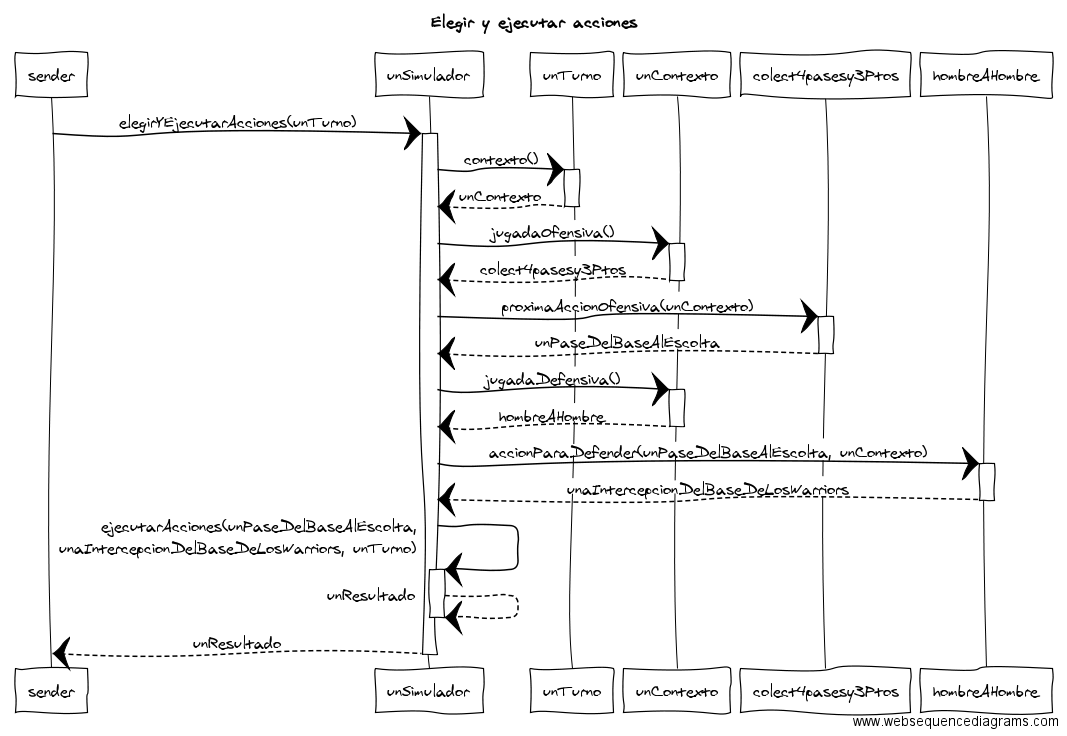
\includegraphics[scale=0.4]{diseno/Elegir_y_ejecutar_acciones.png}
\end{center}
Queda entonces claro cómo es que el simulador se encarga de tomar del \textit{contexto} la jugada que se está realizando, y solicitarle las a ésta las acciones que la conforman para, luego de recibidas, proceder a ejecutarlas.

\subsection{Jugadas y acciones}
A continuación presentamos cómo cada una de las acciones mencionadas en el apartado anterior, se integra con los distintos tipos de jugadas (defensivas/ofensivas/rebote), que a su vez forman parte de los libros de jugadas de los técnicos. Cada \textit{Jugada} usa las \textit{Acciones} que la componen (Pase y Tiro en el caso de las Ofensivas; Bloqueo e Intercepción en el de las Defensivas; y Rebote en el caso de Reboteo).

\begin{center}
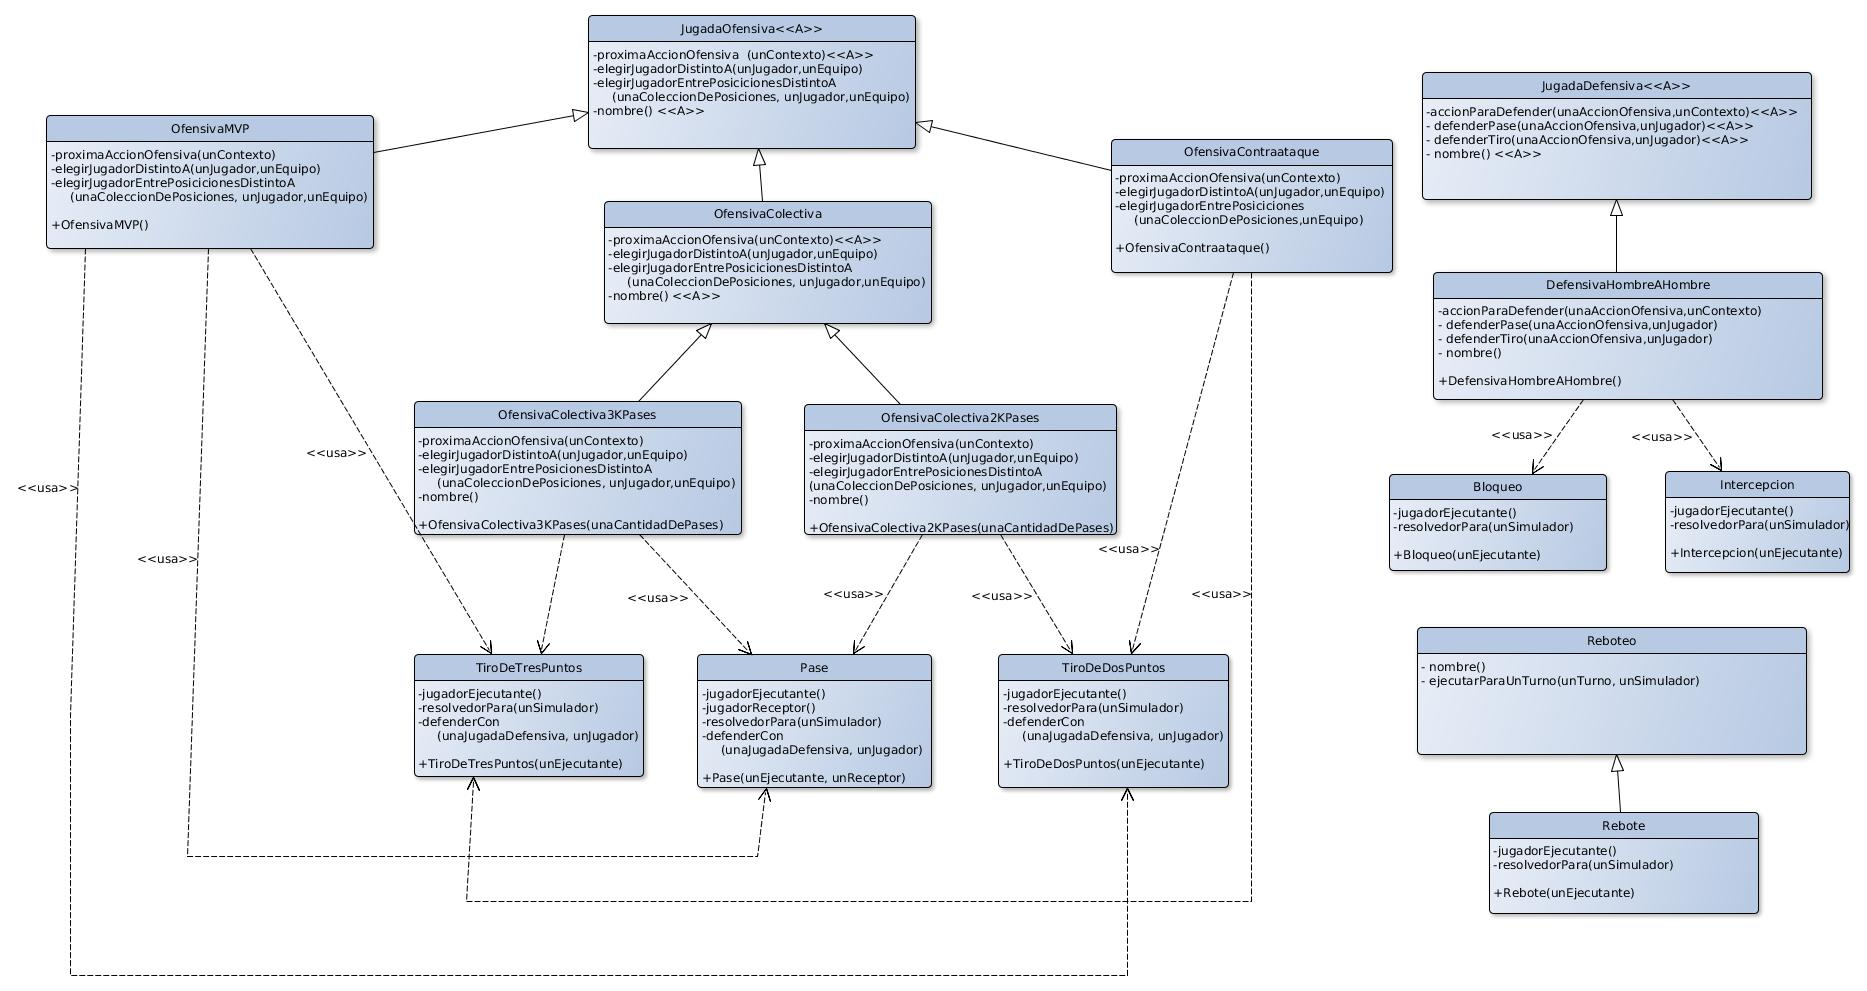
\includegraphics[scale=0.4, angle=90]{diseno/jugadasYAcciones.jpg}
\end{center}

Como mencionamos previamente, la clase abstracta Jugada Ofensiva se subclasifica en tres tipos de jugadas, OfensivaMVP, OfensivaContraataque, y OfensivaColectiva, esta última también abstracta y que se subclasifica en OfensivaColectiva3KPases, y OfensivaColectiva2KPases.

Las jugadas ofensivas son polimórficas. Saben decir, dado un contexto, cuál es la próxima acción ofensiva a ejecutar, y también saben elegir jugadores dentro de un equipo para que formen parte de las distintas acciones (siempre distintos a un jugador pasado por parámetro, y también se los puede buscar entre una lista de posiciones en particular, algo útil en el caso de las jugadas de tipo OfensivaColectiva).

En el caso de las jugadas defensivas, sólo hereda de ella la jugada DefensivaHombreAHombre. No obstante, al seguir el mismo patrón que para JugadaOfensiva, es posible extender la cantidad de jugadas defensivas subclasificando la clase JugadaDefensiva (está claro, siempre y cuando se comporten de manera similar, como una respuesta a una ofensiva; si no, habría que implementar otros métodos).

Modelamos las jugadas defensivas como una respuesta a las jugadas ofensivas. Por esa razón, deben poder responder mensajes con la información de con qué acción defensiva hacen frente a una acción ofensiva. Este mecanismo, de double dispatch, se verá mejor en los diagramas de secuencia presentados a continuación.

A continuación veremos cómo se integran el tecnico con su libro de jugadas para elegir una jugada (en este caso, una ofensiva) con la simulación. Nótese que, dado que las jugadas se eligen en base a la frecuencia de las mismas, se necesitó de un generador de numeros aleatorios para simular el comportamiento de aleatoriedad en la elección de las mismas. \\
(Nota: si bien no aparecen Tecnico y LibroDeJugadas en el diagrama de clases anterior, conceptualmente este diagrama de secuencias tiene más sentido aquí, que en la sección \textbf{3.2.2  - Equipos}, en particular porque la jugada ofensiva se usa en los diagramas posteriores).
\begin{center}
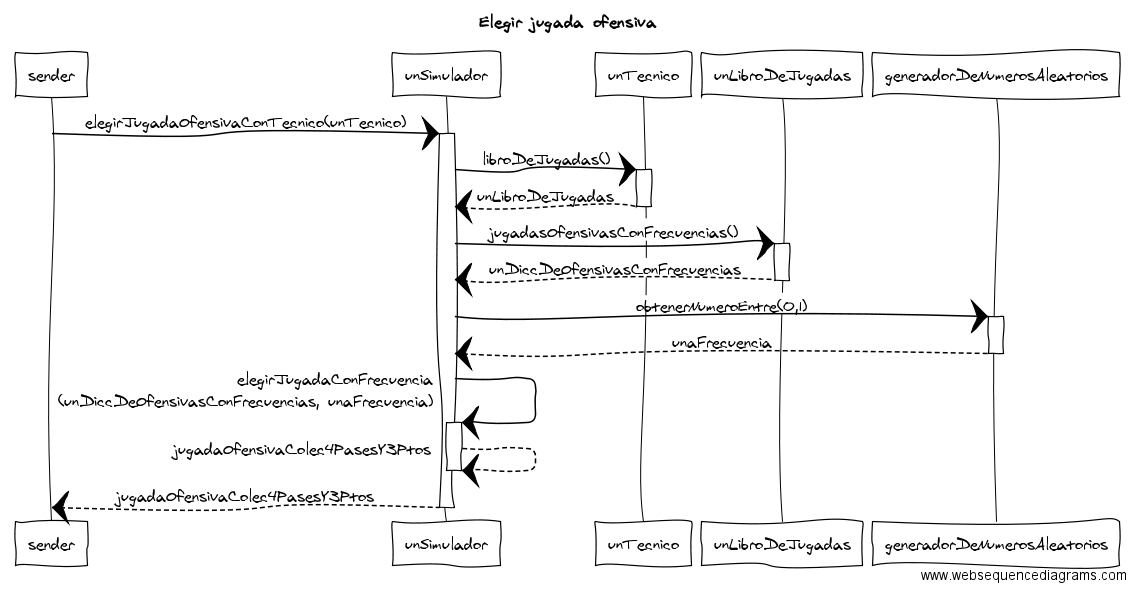
\includegraphics[scale=0.45]{diseno/Elegir_jugada_ofensiva.png} 
\end{center}


El mecanismo para elegir la próxima acción (ofensiva) en una jugada ofensiva es bastante simple. La jugada recibe el contexto del turno como parámetro, y le consulta toda la información que necesita para poder resolver cuál será la próxima acción. Dado que la jugada es de 4 pases, y nos encontramos en el paso 2 (es decir, en el próximo paso no se tirará al aro), la próxima acción será un pase a cualquier jugador del equipo atacante, que no sea el que tiene actualmente la posesión de la pelota. La jugada crea finalmente un pase, con el jugador ejecutante y el jugador receptor, y devuelve esa acción al sender.

\begin{center}
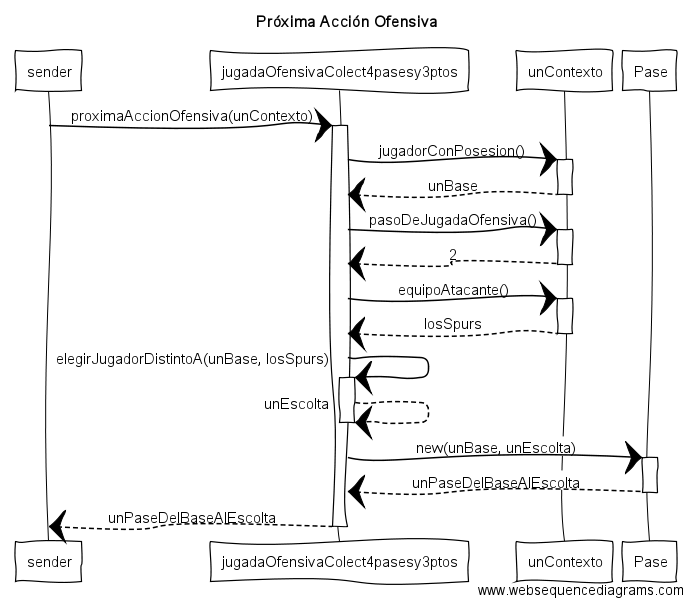
\includegraphics[scale=0.4]{diseno/Proxima_accion_ofensiva.png}
\end{center}

El mecanismo para la próxima acción de una jugada defensiva es más interesante por hacer uso de double dispatch.

Como la jugada defensiva hombre a hombre es siempre en respuesta a una ofensiva, es necesario conocer información de la acción respectiva de la jugada ofensiva que se está ejecutando , y quién es el jugador del equipo atacante en posesión de la pelota, ya que quien realice la acción defensiva deberá ocupar la misma posición, pero en el equipo defensor.

El double dispatch aparece por duplicado, en la interacción entre losWarriors y unaPosicionBase (para saber quién es el jugador de losWarriors que ocupa la posición de base), y luego entre la jugadaDefensivaHombreAHombre y la acción ofensiva unPaseDelBaseAlEscolta (para poder responder de qué manera la jugada defensiva hará frente a la acción ofensiva: mediante una intercepción).

\begin{center}
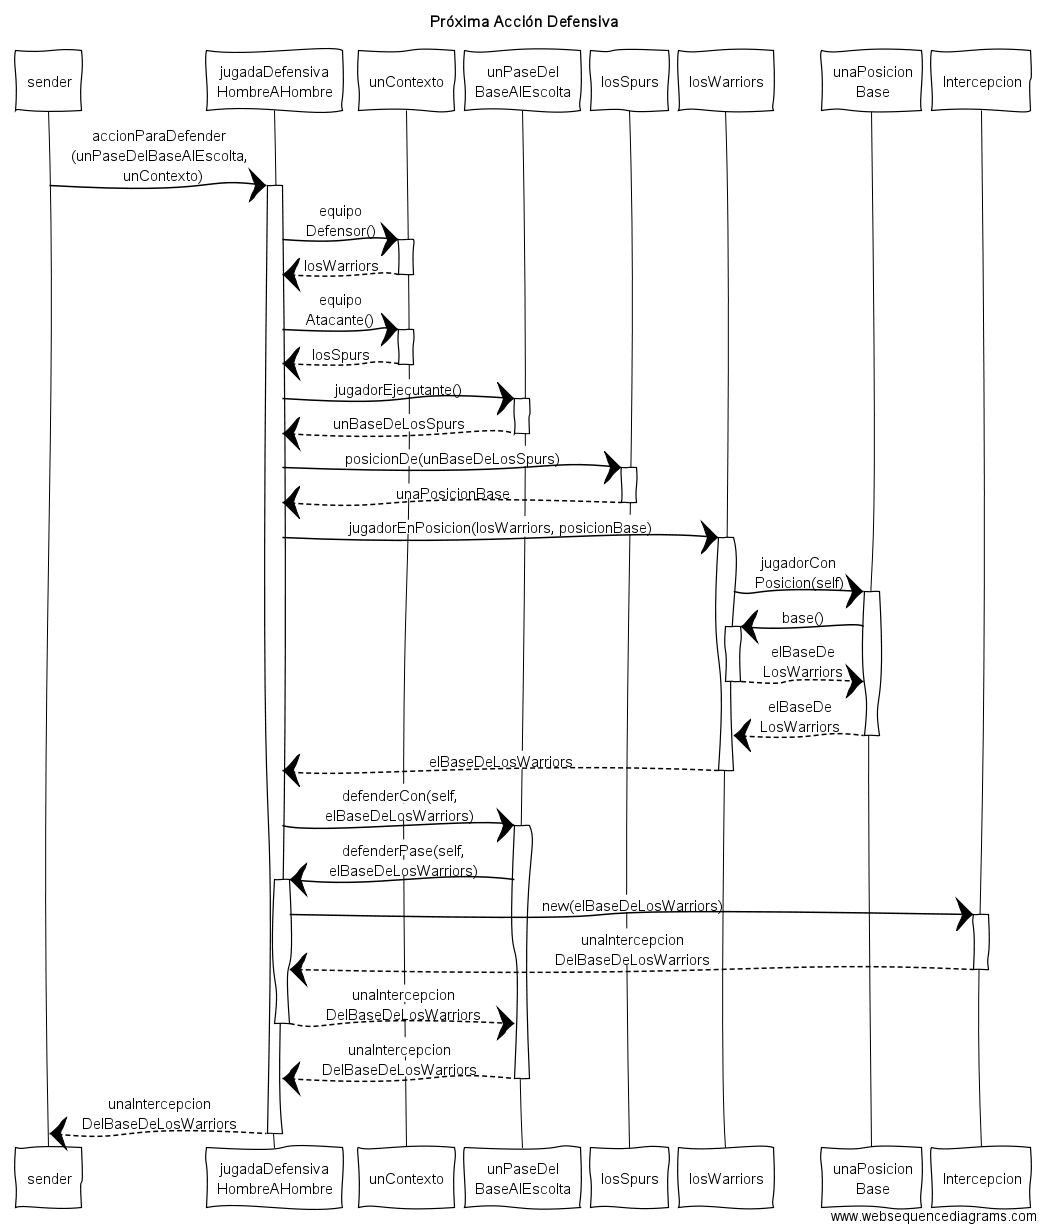
\includegraphics[scale=0.4]{diseno/Proxima_accion_defensiva.png}
\end{center}


\subsubsection{Ejecución de acciones}
En el siguiente diagrama de secuencia se puede apreciar cómo el simulador realiza los pasos de las jugadas en un turno dado. Ya se dispone de una acción ofensiva y de otra ofensiva (elegido en los diagramas previos), por lo que el simulador ejecuta ambas acciones para un turno determinado. A cada una de las acciones le pide su resolvedor correspondiente, a los que les pregunta luego si la acción es exitosa, o no. En base a eso los resultados de las distintas acciones, decide el simulador cómo continúa.

Podemos ver, además, cómo las distintas entidades encargadas de modelar las acciones de una jugada, se relacionan con sus propios resolvedores. En éstos es donde se calculan las probabilidades de éxito y fracaso para todas las acciones de los jugadores. El hecho de que estos cálculos no formen parte de las acciones en sí (además de no ser una solución que conceptualmente nos satisfaciera, puesto que no parecería ser responsabilidad de una acción algo que se corresponde con una simulación/cálculo) agrega un componente de modificabilidad al diseño, puesto que se pueden modificar las ecuaciones encargadas de calcular los resultados de cada acción de manera aislada y sin afectar al resto del modelo.

\begin{center}
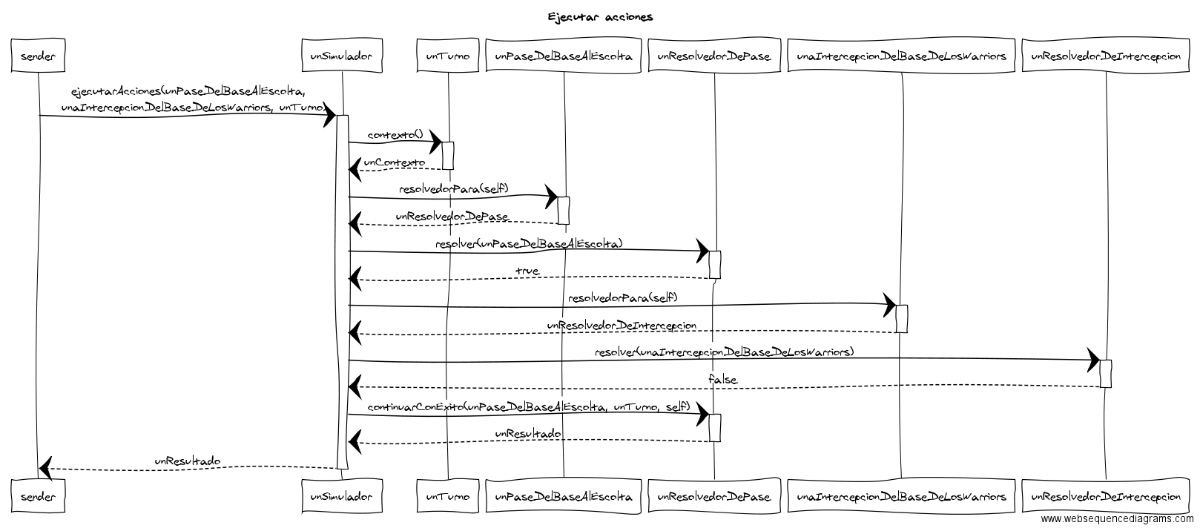
\includegraphics[scale=0.45, angle=90]{diseno/Ejecutar_acciones.png}
\end{center}

\subsubsection{Continuación de acciones}

En el diagrama anterior se ve que una vez que se resolvió si fueron exitosas o no las distintas acciones, el simulador le dice al resolvedor correspondiente cómo debe proceder, si con éxito o con fallo. El resolvedor de cada acción es quien sabe cómo proceder el juego. 

\begin{center}
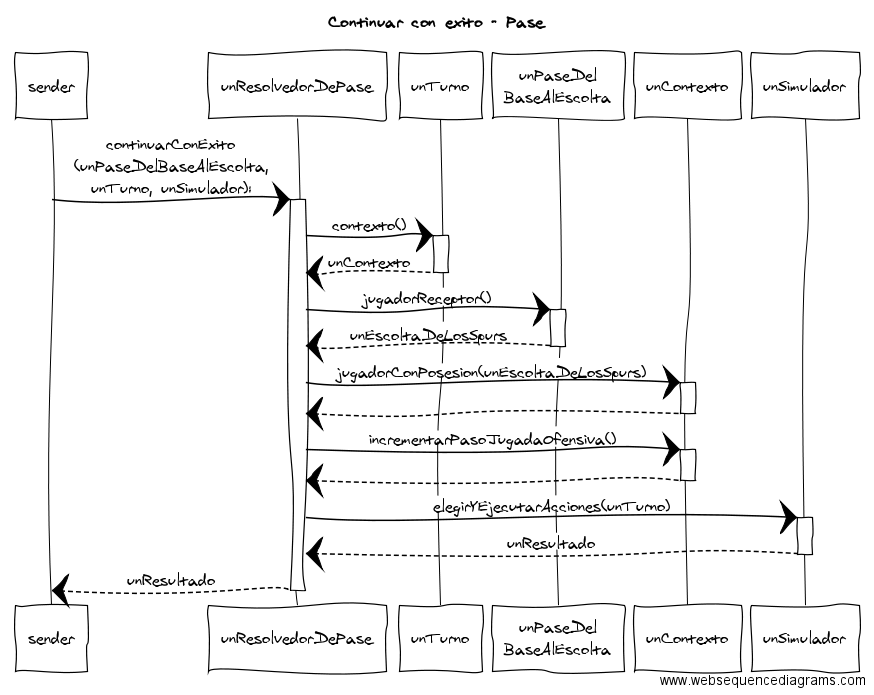
\includegraphics[scale=0.45]{diseno/Continuar_con_exito_pase.png}
\end{center}

Por ejemplo, en el caso de un pase exitoso, le avisa al contexto quién será el nuevo jugador con posesión de la pelota (el receptor del pase), e incrementa el paso de la jugada ofensiva. Finalmente, al tener el turno un nuevo contexto, realiza un llamado recursivo a elegirYEjecutarAcciones(). Eventualmente, cuando el turno llegue a su fin, se retornará un resultado parcial. Por ejemplo, cuando ocurra un tiro exitoso.

\begin{center}
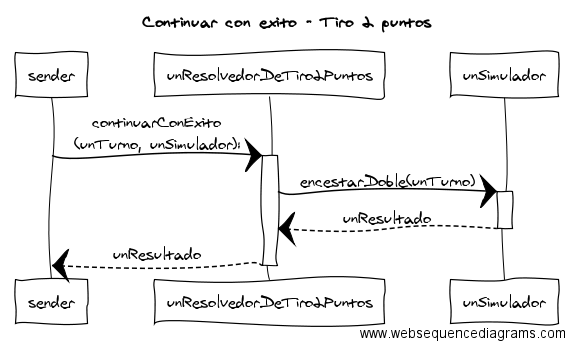
\includegraphics[scale=0.45]{diseno/Continuar_con_exito_tiro_2_puntos.png}
\end{center}

El simulador sabe que cuando ocurre un tiro exitoso y sin intercepción debe procedor el tiro, y el resolvedor le avisa al simulador que debe encestar un doble.

\begin{center}
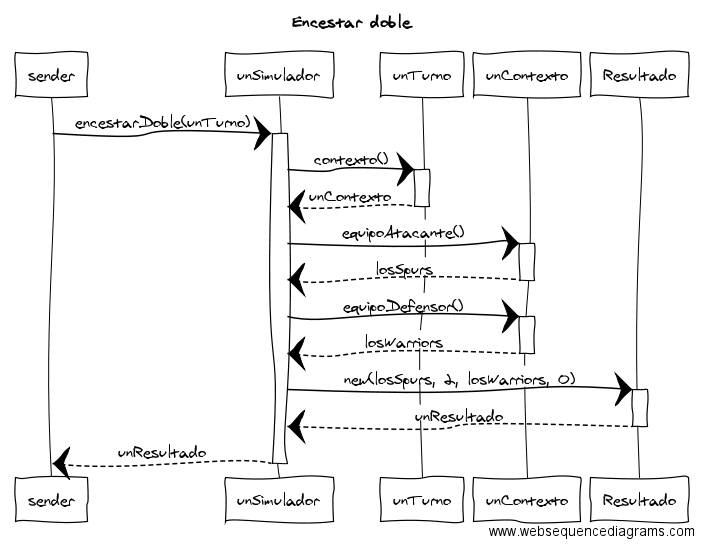
\includegraphics[scale=0.45]{diseno/Encestar_doble.png}
\end{center}

Aquí tenemos un ejemplo de cuándo termina un turno. El simulador crea un objeto de la clase resultado, con el resultado parcial del turno, y devuelve este resultado, que volverá a través de todos los llamados recursivos que se hicieron.


\begin{center}
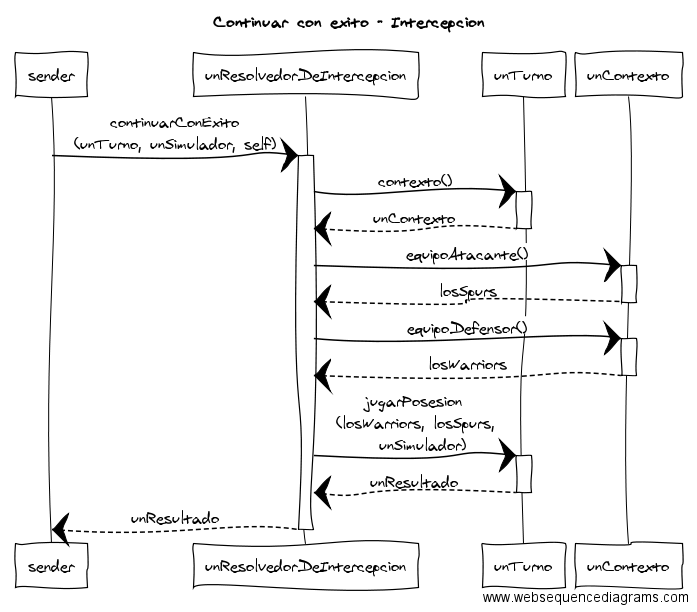
\includegraphics[scale=0.45]{diseno/Continuar_con_exito_intercepcion.png}
\end{center}

Un caso levemente interesante para diagrama de secuencia, es una intercepción exitosa, no porque represente alguna complejidad especial, sino porque llama a jugarPosesion() de unTurno, que es el punto de partida de los turnos. Allí es donde se dice qué equipo es ahora el atacante, cuál el defensor, se eligen las respectivas jugadas, etc.

\subsection{Apuestas}

Modelamos las apuestas con una jerarquía polimórfica simple. La clase abstracta Apuesta se subclasifica en ApuestaNula (haciendo uso del NullObjectPattern), que representa la ausencia de apuesta, y la ApuestaDeFichas, que representa una apuesta en fichas. La razón de ser de la ApuestaNula es la posibilidad de lanzar un desafío sin ninguna apuesta de fichas.\\
\begin{center}
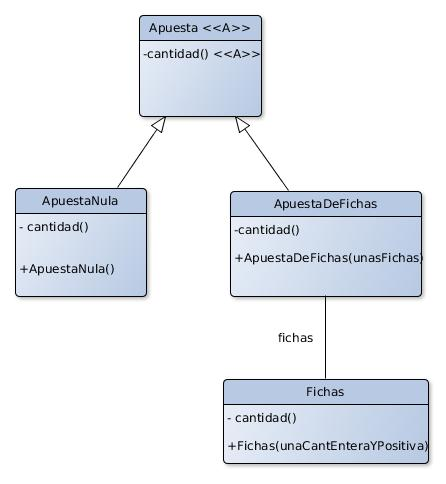
\includegraphics[scale=0.4]{diseno/apuestas.jpg}
\end{center}

\subsection{Gestión de Desafíos}
De la misma manera en que definimos que un participante no conoce si su cap ni sus fichas disponibles, definimos que un jugador no conozca esencialmente los desafíos de los que formó parte.\\
Modelamos entonces una clase GestorDeDesafíos, cuyas instancias no sólo saben los desafíos de un participante, sino que también es se encargan de crear desafíos y de generar el contexto para que se simule un partido de un desafío. Es por esta razón que la clase Gestor de Desafíos usa a la clase Simulador y a la clase Logger.
A su vez, dado que debe indicar las estadísticas de los jugadores para la simuación, conoce al RegistroDeEstadísticas. Dado que debe validar que el participante puede apostar la cantidad de fichas indicadas y además debe actualizar las fichas disponibles de un participante, conoce al GestorDeFichas. Finalmente, como el cap de un participante se puede modificar por el resultado de un desafío, el GestorDeDesafíos conoce al GestorDeCap.\\

Un desafío está representado por la clase Desafío y está compuesto por una apuesta, un EstadoDeDesafío, un participante desafiante y un equipo desafiante.\\
La idea de que un desafío posea un estado representa el hecho de que un desafío puede estar abierto, esperando a ser ejecutado o terminado. Esto se modela a través de la jerarquía de clases EstadoDeDesafio.\\
Aprovechando la existencia de un estado, hicimos uso del patrón de diseño State, proveeyendo un protocolo en común entre un desafío y su estado. De esta forma, podemos modificar el comportamiento del desafío en runtime y, por ejemplo, modelar que no se puede simular un desafío abierto, ni se le puede pedir un resultado a un desafío en ejecución. El estado conoce al desafío al que conoce, de manera tal de poder enviarle el mensaje para cambiar de estado.\\
El estado EstadoDeDesafioAbierto, solo responde al mensaje incribirDesafiado(unParticipante, unEquipo), a partir del cual instancia el EstadoDeDesafioEnEjecucion como corresponde con los datos del desafiado y le envía el mensaje para cambiar de estado al desafío con el nuevo estado instanciado. Para todos lo demás mensajes lanza una excepción.
Análogamente, el EstadoDeDesafioEnEjecucion responder al mensaje realizarCon(unSimulador, unLogger) a partir del cual instancia un Partido y ejecuta la simulación. Finalmente, con los datos que poseía más el resultado del Partido, instancia un EstadoDeDesafioTerminado y le envía el mensaje de cambiar de estado al desafío a EstadoDeDesafioTerminado. Además responder a los mensajes desafiado() y equipoDesafiado(). Para todos los demás mensajes lanza una excepción.
Finalmente el EstadoDeDesafíoTerminado responde solamente a los mensajes ganador(), perdedor(), resultado(), desafiante(), equipoDesafiante() y para todos los demás mensajes lanza una excepción.

A través del GestorDeDesafíos se puede lanzar un desafío a través del mensaje incribirDesafío(unParticipante, unEquipo, unaApuesta). El GestorDeDesafíos, al recibir este mensaje, valida que la apuesta pueda realizarse para el participante y que el equipo pertenezca al participante desafiante. Luego, genera una nueva instancia de Desafío con el participante como desafiante, el equipo como equipo desafiante y la apuesta como la apuesta y con EstadoDeDesafíoAbierto.\\
Análogamente, mediante el mensaje aceptarDesafio(unParticipante, unEquipo, unDesafio) busca el desafío en cuestión, valida que el participante pueda realizar la apuesta y que el equipo perteneza al participante y luego le envía al desafío el mensaje incribirDesafiado(unParticipante, unEquipo) que lo reenviará a su estado.\\
Finalmente, mediante el la recepción del mensaje realizarDesafio(unDesafio), el GestorDeDesafios busca el desafío.Si lo encuenta, instancia un Simulador y un Logger y le envía al desafío el mensaje realizarCon(unSimulador, unLogger), que será reenviado a su estado.\\

El GestorDeDesafios además responde a los mensajes desafiosAbiertos(), desafiosFinalizados(), desafiosDe(unParticipante), desafiosAbiertosDe(unParticipante), desafiosGanadosPor(unParticipante), desafiosPerdidosPor(unParticipante), que no hacen más que filtrar los desafíos que se corresponden con los parámetros de búsqueda y los devuelve en una colección.\\

\begin{center}
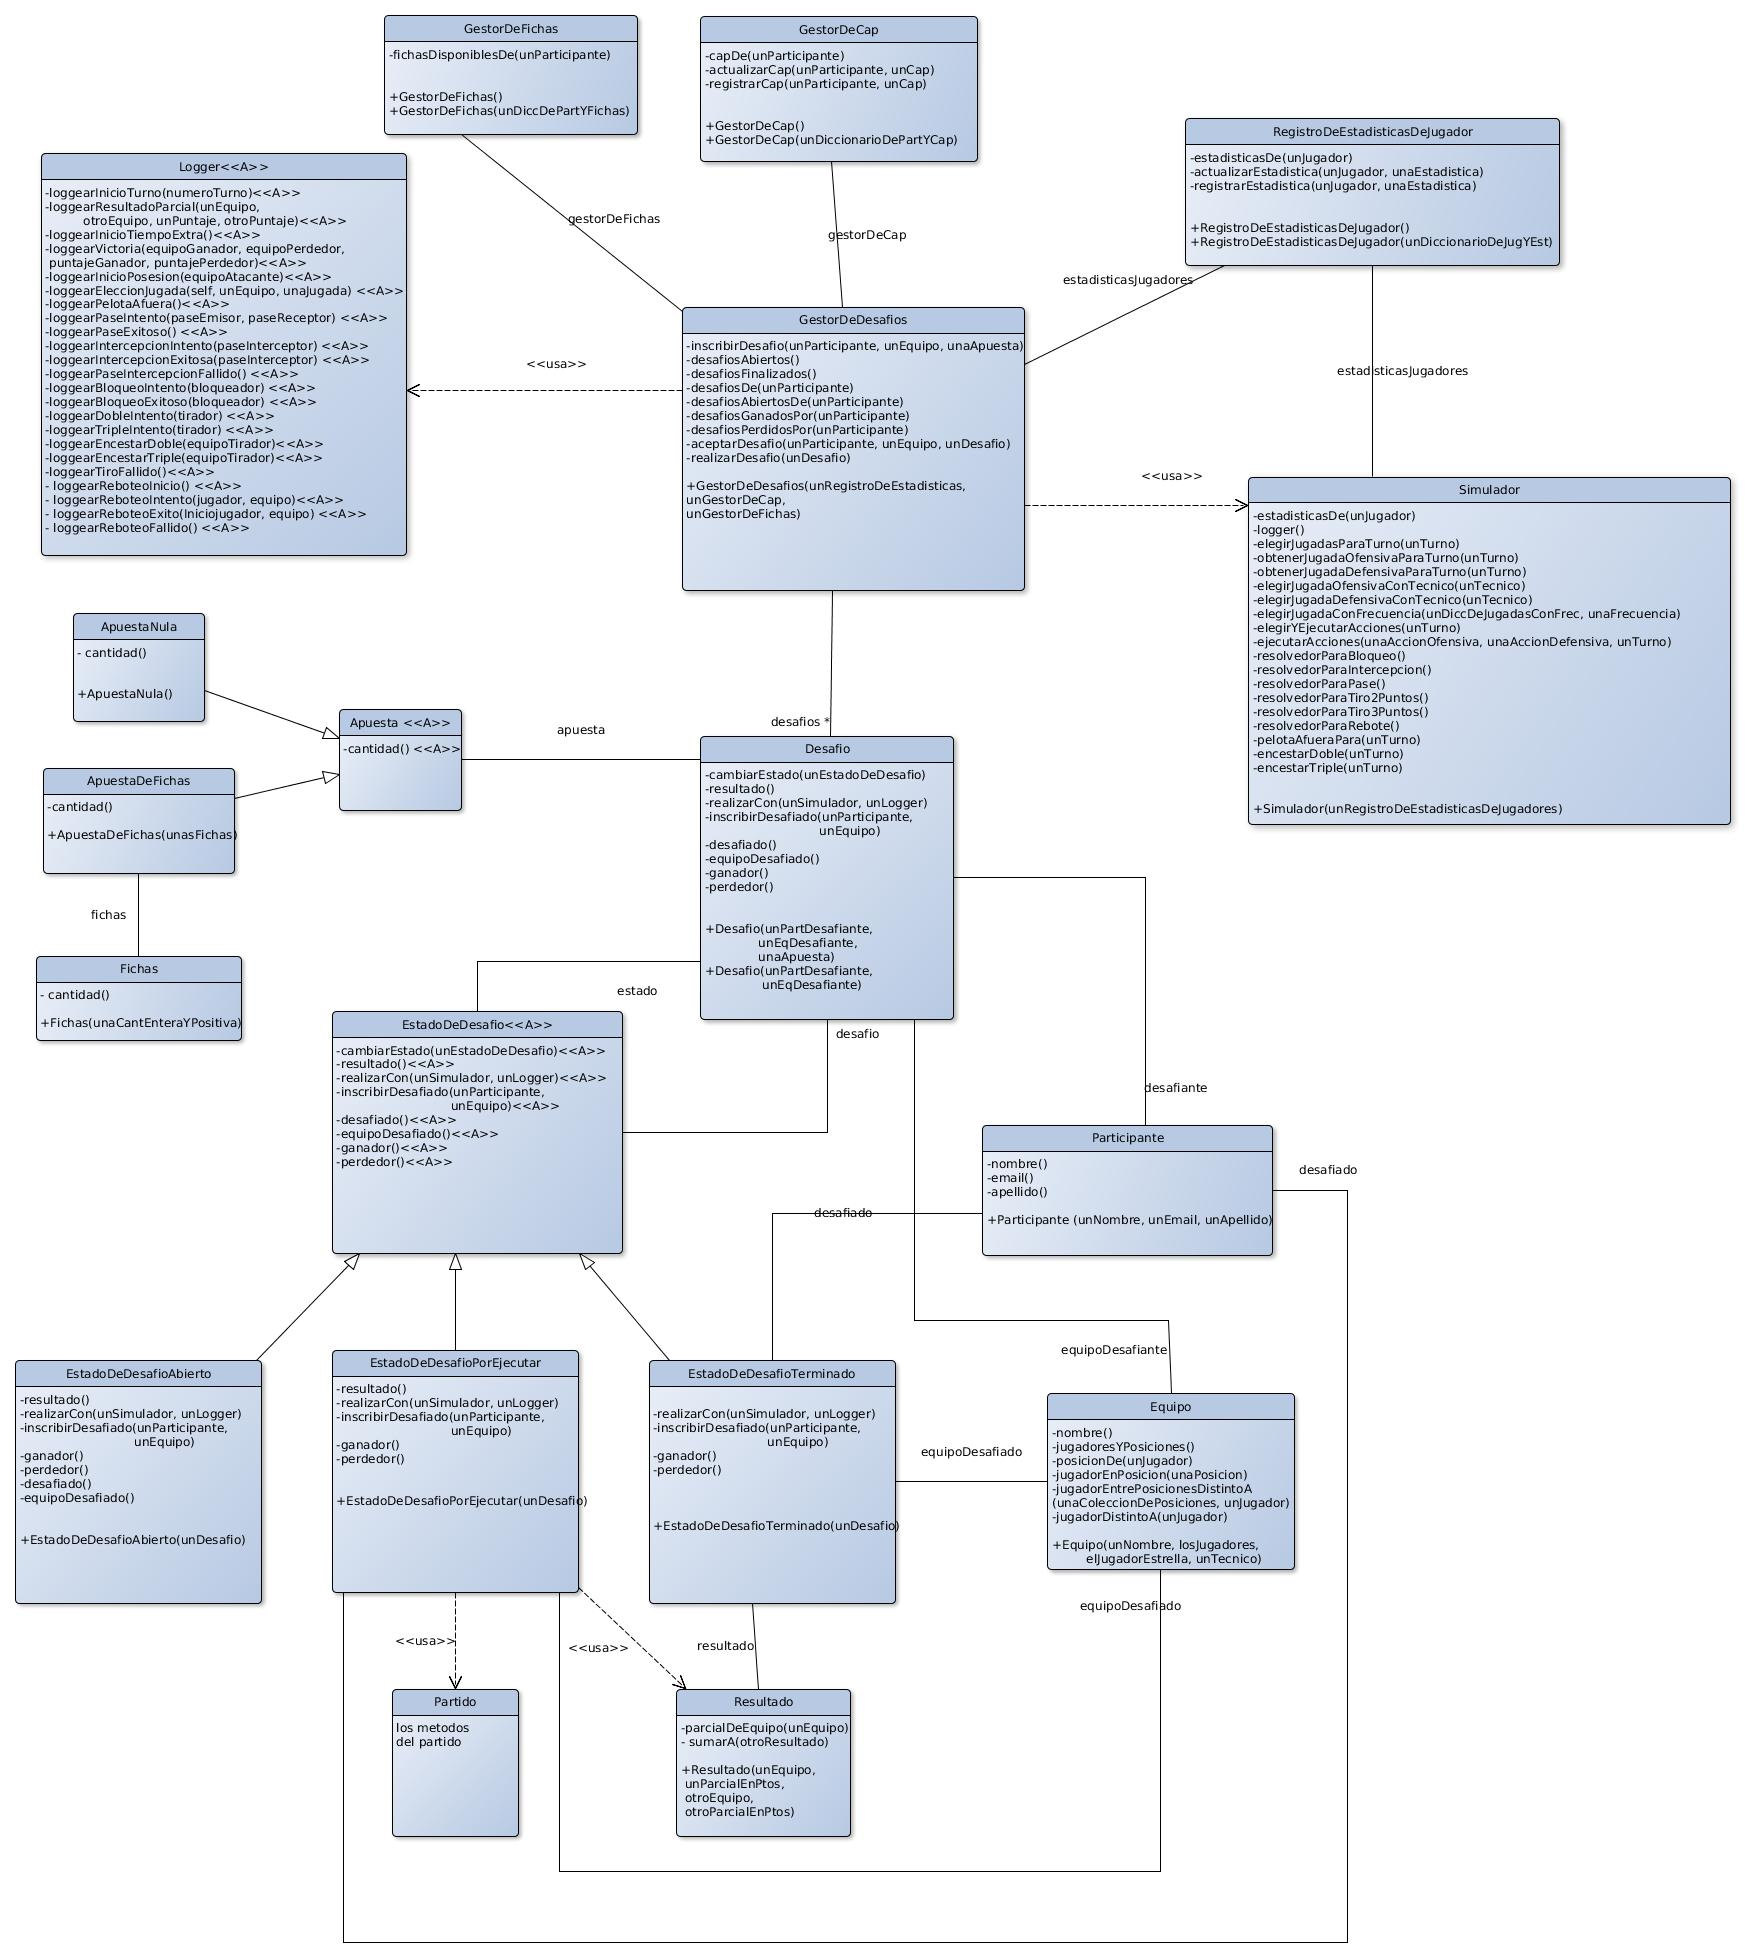
\includegraphics[scale=0.35]{diseno/gestionDeDesafios.jpg}
\end{center}


\subsection{Partido}
\begin{center}
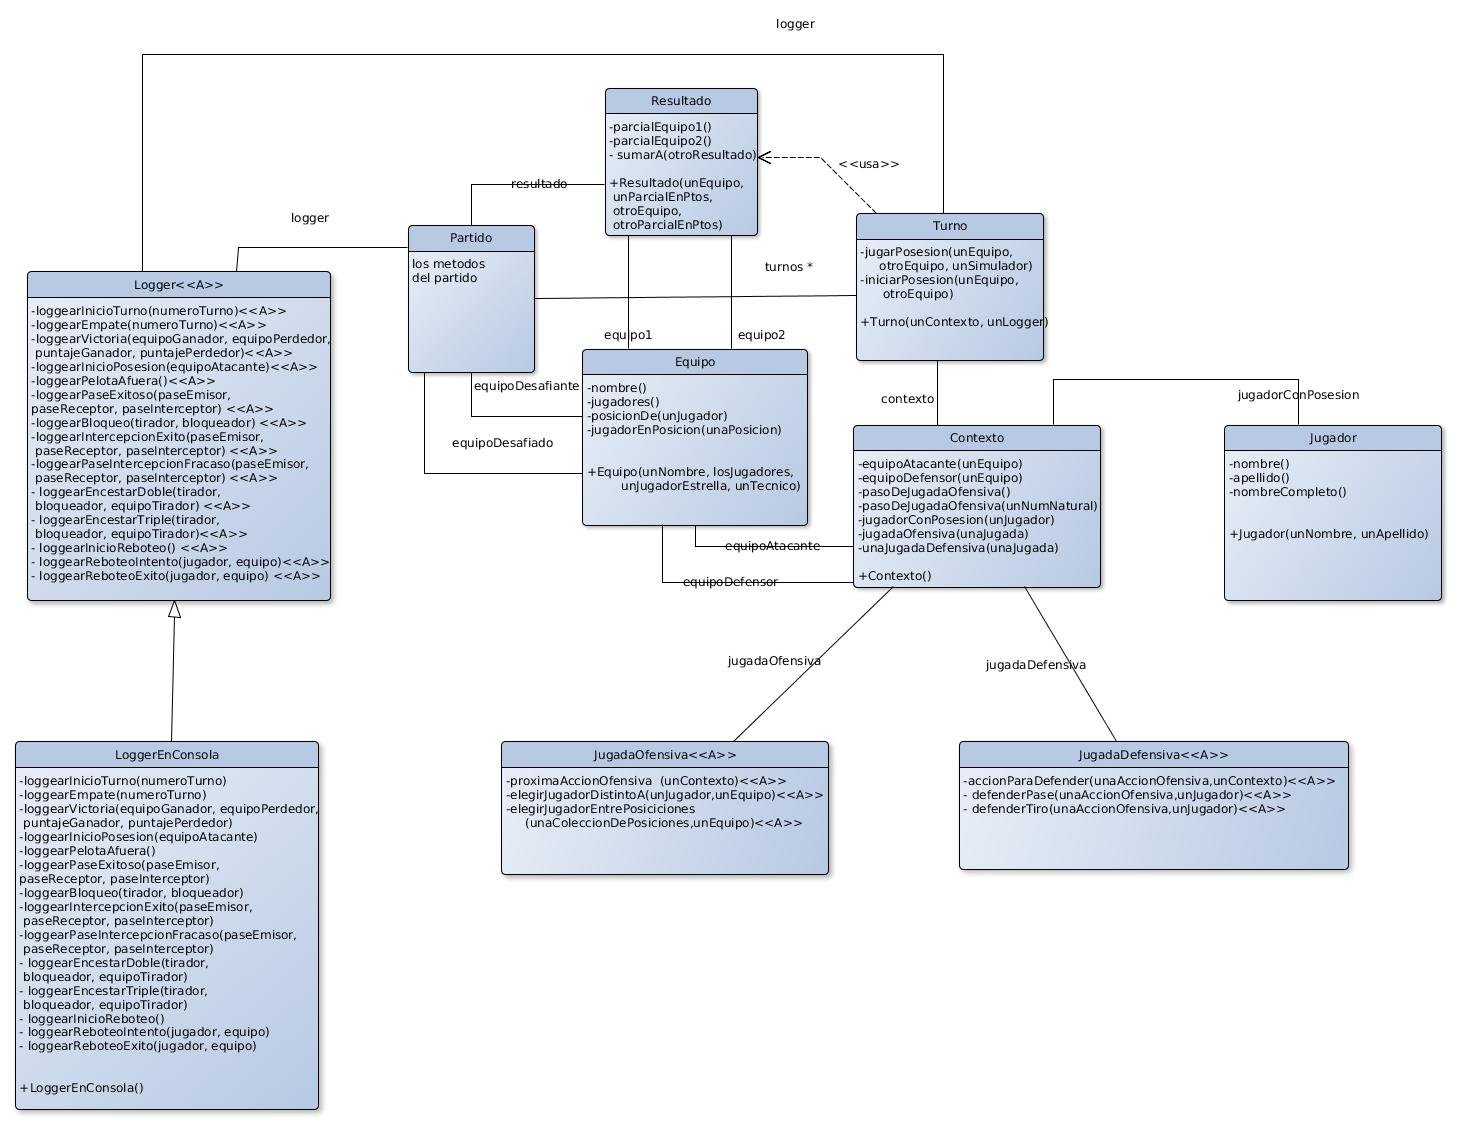
\includegraphics[scale=0.4, angle=90]{diseno/partido.jpg}
\end{center}
Analicemos ahora el diagrama de clases de las entidades que componen un partido. Podemos ver, en un planteo un poco más general, cómo se realiza tambien el loggeo de las distintas acciones que realizan los jugadores, y cómo se integra la entidad Resultado para poder dar cuenta de cómo finalizan las distintas acciones que mencionamos en secciones anteriores. 

Todo el loggeo de las distintas acciones se realiza mediante una clase abstracta que permite que en un futuro, en lugar de imprimir la salida por consola como sucede actualmente, el output donde se loggeen los resultados pueda ser alterado (por ejemplo, que escriba a un archivo) con un mínimo impacto en el resto del sistema, disminuyendo la complejidad.

El partido comienza con el llamado a JugarCon(), donde un partido comienza a jugar con un simulador y logger dados. Al partido le interesa tener conocimiento de cuál es el último equipo que empezó un turno (para poder invertirlos en el próximo turno; cabe destacar que esta información no se puede sacar del Contexto, ya que el equipo atacante/defensor puede no ser el mismo que sacó en el Turno), qué equipo va ganando y cuál no va ganando, y si el partido está empatado (en cuyo caso se debería \textbf{jugarTiempoExtra()}), 

Es el partido el que va creando los distintos turnos, les da un contexto, y va acumulando los resultados parciales de cada uno. Luego de crear cada turno, el partido llama a jugarPosesion(), donde estipula qué equipo sacará y qué equipo no saca, y a partir de allí se eligen las jugadas para cada turno, y las acciones. Notar también que jugarPosesion() es el método al que se llama cuando hay un cambio de posesión en un mismo turno (con una intercepción exitosa, o en un reboteo), es posible usarlo en ambos ámbitos sin ningún problema.

\begin{center}
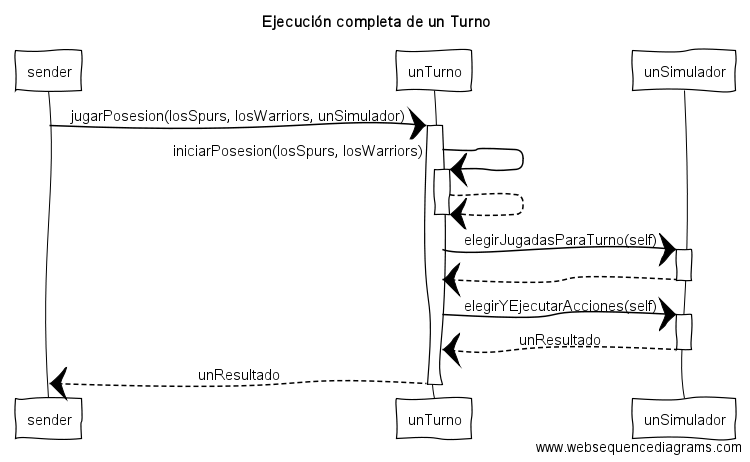
\includegraphics[scale=0.4]{diseno/Ejecucion_completa_de_un_turno.png}
\end{center}


